\documentclass[acmtocl]{acmtrans2m}

\usepackage{graphicx}
\usepackage{subfigure}

\newtheorem{theorem}{Theorem}[section]
\newtheorem{conjecture}[theorem]{Conjecture}
\newtheorem{corollary}[theorem]{Corollary}
\newtheorem{proposition}[theorem]{Proposition}
\newtheorem{lemma}[theorem]{Lemma}
\newdef{definition}[theorem]{Definition}
\newdef{remark}[theorem]{Remark}

\newcommand{\subscale}{0.50}
\newcommand{\mainscale}{1}

\newcommand{\comment}[1]{}

\title{An Experimental Study of Sorting and Branch Prediction}

\author{
PAUL BIGGAR
\and
DAVID GREGG
\\University of Dublin, Trinity College
}

\begin{abstract}

\end{abstract}

\category{E.5}{Data}{Files}[Sorting/Searching]
\category{C.1.1}{Computer Systems Organization}{Processor Architectures, Single Data Stream Architectures}[Pipeline architectures]
\terms{Algorithms, Experimentation, Measurement, Performance}
\keywords{Sorting, Branch prediction}

\begin{document}

\begin{bottomstuff}
Corresponding author's address: David Gregg, Department of Computer
Science, University of Dublin, Trinity College, Dublin 2, Ireland. {\tt
David.Gregg@cd.tcd.ie}.
\end{bottomstuff}

\maketitle

\section{Motivation}
Classical analyses of algorithms make simplifying assumptions about
the cost of different machine instructions. For example, Knuth's Mix
machine code assumes that all operations have unit costs. More
recently researchers have recognized that on modern computers the cost
of accessing memory can vary dramatically depending on whether the
data can be found in the first-level cache, or must be fetched from a
lower level of cache or even main memory.  This has spawned a great
deal of research on cache-efficient searching and sorting \cite{}.

Another type of instruction whose cost can vary dramatically is the
conditional branch. Modern pipelined processors depend on \emph{branch
prediction} for much of their performance.  If the direction of a
conditional branch is correctly predicted ahead of time, the cost of
the conditional branch may be as little as the cost of, say, an
integer add instruction. If, on the other hand, the branch is
mispredicted the the processor must flush its pipeline, and restart
from the correct target of the branch. This cost is typically a large
multiple of the cost of executing a correctly-predicted branch. For
example, the Intel Pentium 4 processor has a 31-stage pipeline,
meaning that a branch misprediction will cost around 30 cycles.  In
contrast, on the same processor the cost of a memory access that
misses the first level cache and hits the second level cache is 23
cycles. Fortunately, the branches in most programs are very
predictable, so branch mispredictions are usually rare (prediction
accuracies of greater than 90\% are typical).

The cost of executing branches is particularly important for sorting
because the inner loops of most sorting algorithms consist of
camparisons of items to be sorted. Thus, the predictability of
these comparison branches is critical to the performance of
sorting algorithms. In this paper we study the predictability
of branches is most of the major sorting algorithms. We also
examine cache-conscious variations of some of the algorithms,
and show how optimizations for the cache impact in branch
mispredictions.



The rest of this paper is organized as follows.

\section{Branch prediction}

\section{Experimental setup}

\section{Elementary sorts}
\label{ordernsquared}
Elementary sorts are also referred to as $O(N^2)$ sorts. These
algorithms have the worst performance for large inputs. However they
have two advantages: they are simple to implement correctly and they
are often faster than more sophisticated algorithms for small input
sets. Four of these sorts are discussed here: selection sort,
insertion sort, bubblesort and shakersort.

Selection sort is a simple algorithm that repeatedly finds the
smallest element of the array and removes it to a sorted section at
the start. It requires approximately $N^2/2$ comparisons and exactly
$N$ exchanges. Insertion sort takes a different strategy and instead
creates an (initially empty) sorted region at the start of the array
and inserts items into their correct position in this sorted region.
Insertion sort performs in linear time on a sorted list. With a random
list, there are, on average, there are $N^2/4$ comparisons and $N^2/4$
half-exchanges. Thus, selection sort performs around twice as many
branches as insertion sort.

Although we know the approximate number of comparisons that each
algorithm performs, and important question is whether there is any
difference of the predictability of the branches in each algorithm.
Figure \ref{Predictability-of-insertion-and-selection-sorts} shows the number of mispredictions per key for both the
algorithms using random data, and varying data set sizes, measured
using the Simplescalar processor simulator.

\begin{figure}[h]
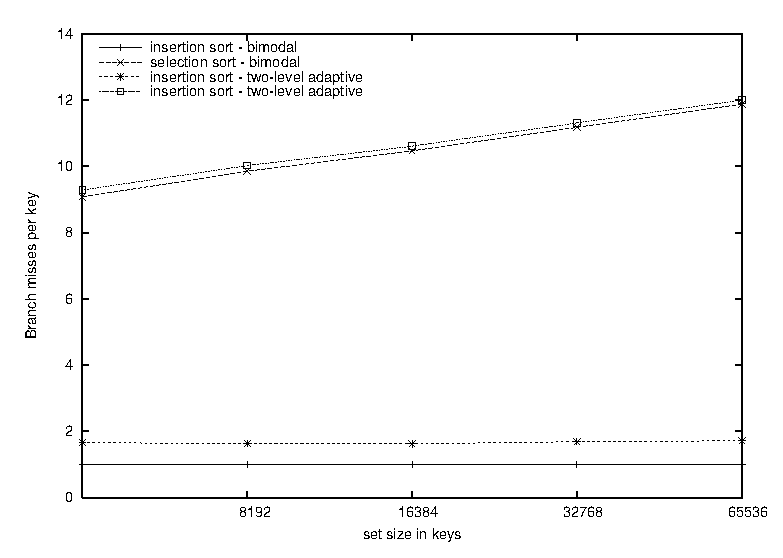
\includegraphics[scale=\mainscale]{plots/bpred_misses_insert_select.eps}
\caption{TODO: Predictability of insertion and selection sorts}
\label{Predictability-of-insertion-and-selection-sorts}
\end{figure}

There are three notable features in this data. Firstly, the number of
mispredictions is very low. If the behaviour of these branches were
random, then we would expect that half of the comparison branches
would be mispredictions, that we would expect $O(N^2)$
mispredictions. In fact, the number of mispredictions per key is less
than 12 even for the largest arrays. Secondly, although selection sort
performs twice as many comparison branches it does not cause twice as
many branch mispredictions. For the bimodal predictor, it causes 9-12
times as many mispredictions within the size of input sets that we
examine. Thirdly the two-level branch predictor is slightly worse at
predicting the comparison branches in these algorithms than the simple
bimodal predictor.  This is a remarkable result, because two-level
predictors are similar to, or sigificantly more accurate than bimodal
predictors for almost all other types of branches \cite{Uht}.

\subsection{Insertion sort}
With a bimodal predictor, insertion sort causes almost exactly one
branch misprediction per key, regardless of the size of the array.
Thus, although insertion sort performs around $N/4$ comparisons per
key, only one of these comparisons causes a misprediction. The
reason for this becomes clear when we consider the inner loop
of insertion sort:
\begin{verbatim}
   while( item < a[j-1] ) {
     a[j] = a[j-1];
     j--;
   }
   a[j] = item;
\end{verbatim}

The comparison in insertion sort is also the loop guard.  As long as
the loop continues, this comparison always resolves in the same
direction, and is thus highly predictable. When the location for the
item is finally found, the comparison resolves in the opposite
direction, and a branch misprediction occurs. Thus, for a bimodal
predictor, the number of mispredictions per key is almost exactly
one. Although the results we present are for random data, the same
is true regardless of the input data. Insertion sort will always
cause around one misprediction per key.

The two-level predictor combines a pattern of recent branch outcomes
make a prediction. This goal is to exploit correlations between branch
outcomes. For most programs this is valuable, but there is correlation
of branch outcomes in insertion sort. The additional complexity simply
causes the predictor to find false correlations, with the result that
number of mispredictions is higher than for a simpler, bimodal
predictor. In general, misprediction rates of more than one per key
are caused by imperfections in the predictor, rather than the
unpredictability of the comparison branch in insertion sort.

\subsection{Selection sort}
The comparison branch in selection sort is also highly predictable,
but less so than for insertion sort. The inner loop of selection
sort consists of searching for the smallest element of part of
the array:
\begin{verbatim}
  min = i;
  for ( j = i+1; j < N; j++ )
    if ( a[j] < a[min] ) min = j;
\end{verbatim}
The predictability of the comparison branch depends on the number of
times that the cadidate minimum, $min$, changes. Knuth \cite{Knuth97}
shows that for $N$ elements, the number of changes is $H_N - 1$, where
$H_N$ is the harmonic series:
$$H_N = 1 + \frac{1}{2} + \frac{1}{3} + ... + \frac{1}{N} =  \sum_{k=1}^{N}
\frac{1}{k},  \hspace{0.4cm}  N \geq 1$$

Within practical sorting ranges, $H_N$ grows at a rate similar to
$log_e(N)$. Thus, in the average case, we can expect that the comparison
branch will mostly go in the same direction, making the branch highly
predictable.

The number of changes to the left-to-right minimum in the best case is
zero and in the worst case $N-1$. In the worst case, the array is
sorted in reverse order, and so the left-to-right minimum changes on
every element. Interestingly, the worst cases for the number of
changes is not the worst case for branch mispredictions. If the
minimum changes for every element, then the comparison branch will
always resolve in the same direction, and thus be almost perfectly
predictable. From the point of view of branch prediction, frequent
changes (preferably with no simple pattern) are the main indicator of
poor performance, rather than the absolute number of times that the
branch resolves in each direction. The worst case for selection sort
would be an array which is partially sorted in reverse order; the
left-to-right minimum would change frequently, but not predictably so.

\subsection{Bubble sort}
Bubblesort is a notoriously inefficient algorithm that compares and
exchanges adjacent pairs of elements in the array. One execution of
the inner loop will move the smallest element of the array to the
first position, and partially sort the rest of the array by moving
small elements towards the start. Cocktail shaker sort (or simply
shakersort) alternates the direction of the inner loop to take
more advantage of this partial sorting to reduce the number of
outer-loop iterations.

Figure \ref{Predictability-of-bubblesort-and-shakersort} shows the number of branch mispredictions per key for
bubble- and shakersort.  Nearly one in four comparisons in bubblesort
are mispredicted. As the data sets gets large, there are nearly 10000
branch mispredictions per key key. Shakersort executes a lot fewer
branches, and so has fewer mispredictions, but the rate of
misprediction is similar.

\begin{figure}[h]
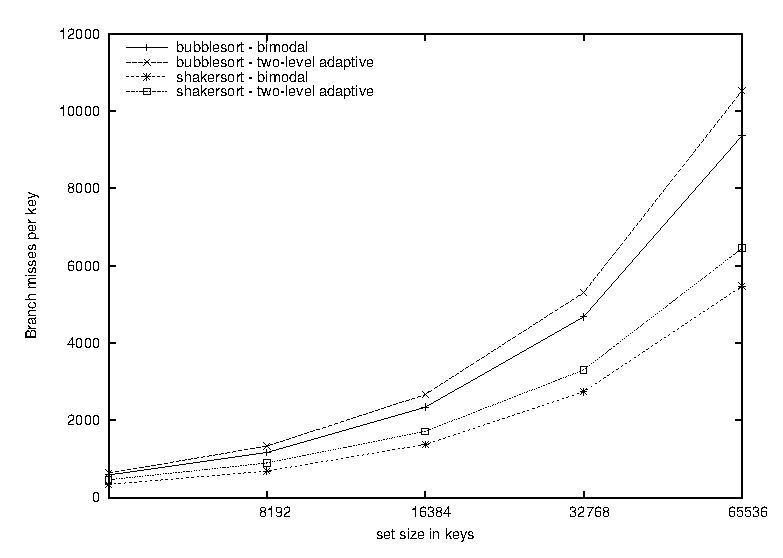
\includegraphics[]{plots/bpred_misses_bubble_shaker.eps}
\caption{TODO: Predictability of bubble and shaker sorts}
\label{Predictability-of-bubblesort-and-shakersort}
\end{figure}

The branch behaviour of bubblesort is particularly interesting when
compared to selection sort. Although we usually think of the two
algorithms as being different, they are actually very similar. Like
selection sort, bubblesort finds the smallest key in the
unsorted part of the array and moves it to start of the
array. Thus, we would expect that bubblesort's branch prediction
behaviour would be similar to that of selection sort.

However, in the process of moving the smallest element into position,
bubblesort also rearranges other array elements. Selection sort sweeps
across the array and always keeps track of the left-to-right minimum
up to the current point.  However, bubblesort actually moves this
minimum, exchanging pairwise with each element it encounters which is
larger. Thus, even the unsorted part of the array becomes partially
sorted. We might expect that bubblesort's comparison branch for a
partially sorted array might be more predictable than for a random
one, but it is not. With a random array, the smaller elements are
equally likely to appear anywhere in the array. With a partially
sorted array, the smaller elements tend to appear towards the start of
the array which is, in bubblesort, the last place that we look. Thus,
the candidate minimum is changed much more often than if we were
searching a randomly ordered array.

\begin{figure}[h]
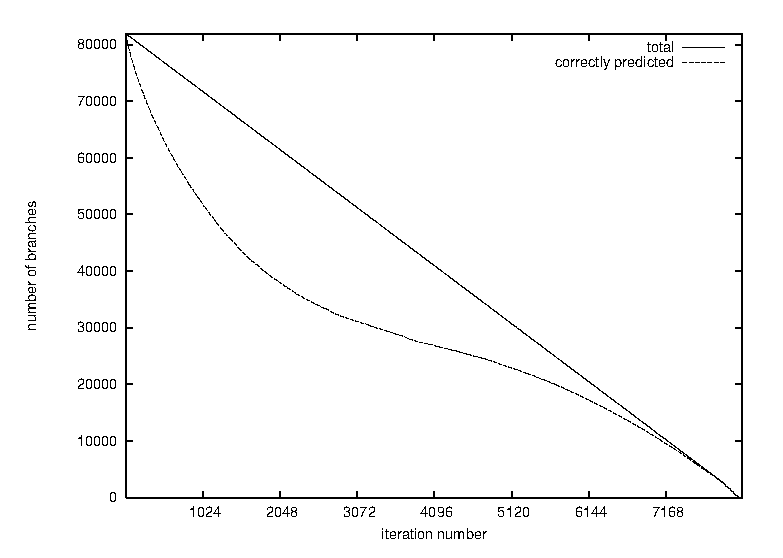
\includegraphics{plots/bpred_bubble_progress.eps}
\caption{Behaviour of branches in bubblesort compared to the ``sweep'' number}
\label{Predictability-of-branches-in-bubblesort-compared-to-sweep-number}
\end{figure}

To demonstrate this effect, we measured how the predictability of
bubblesort's comparison branch varies with successive sweeps across
the array. We added a simple software simulation of a bimodal
predictor to the source code of base bubblesort, and ran it on a large
number of randomly generated arrays, each with 8192 elements.

Figure
\ref{Predictability-of-branches-in-bubblesort-compared-to-sweep-number}
shows that on the early iterations the number of correct predictions
is very close to the number of executed comparison branches. The
comparison branch is highly predictable because bubblesort's search
for the smallest element is similar to selection sort. However, with
successive sweeps even the unsorted part of the array becomes
increasingly sorted and the branch becomes more unpredictable. We see
that the number of executed comparison branches falls linearly, but
that the number of correctly predicted comparison branches falls much
more quickly. Eventually, the array becomes so close to fully sorted
that the branch becomes increasingly predictable in the other
direction, and the number of correct predictions again approaches the
number of executed branches. However, during the intermediate stage,
a huge number of branch mispredictions have already
occurred. Paradoxically, by partially sorting the array, bubblesort
greatly increases the number of branch mispredictions and thus greatly
increases its running time.

Overall, our results show that branch prediction is an important
factor in the efficiency of sorting algorithms. For example,
shakersort executes fewer machine instructions and causes fewer cache
misses than selection sort, but is slower due to branch
mispredictions. Insertion sort is confirmed as the most efficient
elementary sorting algorithm. In additon to having the best time
complexity it causes only around one branch misprediction per key even
in the worst case.

\section{Shellsort}
Shellsort \cite{Shell59} was the first in-place sub-$N^2$ sorting
algorithm. The algorithm operates by sorting all elements that are $h$
elements apart using insertion, where $h$ is some increment.  On early
iterations the increment is large, allowing items to move large
distances. The increment is reduced on successive iterations to allow
more local sorting. The final iteration is a standard insertion sort,
after which the array is sorted. We use Gonnet's increments, which set
the next value of the increment to $\frac{5}{11}^{th}s$ of the
previous increment, because we found them to be efficient in practice.
All discussions of complexity are based on these increments.

The branch performance of shellsort should be predictable. There are
$log_{(\frac{11}{5})}N$ increments, each with a separate pass over the
array. On each pass, all keys are insertion sorted into some
sub-array. Given that insertion sort causes around one branch
misprediction per key, we can expect $N$ comparison branch
mispredictions per pass. It is expected, therefore, that there will be
around $log_{(\frac{11}{5})}N$ mispredictions per key. In general, if
there are $i$ increments, shellsort will cause $ni$ mispredictions.

Figure \ref{} shows the number of branches and branch mispredictions
per key for shellsort. For 4194304 keys, we would expect
$log_{(\frac{11}{5})}4194304 = 18.34$ mispredictions per key. The
number of mispredictions we measure in our simulation is actually a
little under 18, which is remarkably close to the predicted number.

To further investigate this we separated the comparison branches from
the other branches in the code in a separate simulation of a bimodal
branch predictor on a large number of randomly generated arrays. We
found that using Gonnet's increments each key moves only an average of
0.9744 places in each insertion sort (although moving one place
actually involves skipping over $h$ other array elements, where $h$ is
the increment). Thus, the situation is somewhat different to insertion
sorting large arrays of random elements where each element can be
expected to move a large number of places. Instead of the comparison
branch almost always resolving in one direction, the actual outcome
will be close to random. We can still expect a number of
mispredictions that is close to one per key, but we are unlikely to
get the almost perfectly predictable behaviour that we see when using
insertion sort where the average number of places moved is larger.

The main apparent weakness of shellsort on modern architectures is its
poor locality of reference in memory access.  By comparing items which
are separated by $h$ keys, there is little reuse of items in the same
cache line. One can easily imagine cases where shellsort would cause
very large numbers of cache misses.  In the worst case, each key would
move a very large number of places in each insertion sort pass,
possibly causing a cache miss for every place that it moves.  To
further investigate this effect, we measured the number of first and
second-level cache misses caused by our implementation of shellsort
(see figure \ref{Cache-misses-in-shellsort}). In fact, the number of mispredictions caused by
our shellsort is significant, but not much greater than other sorting
algorithms such as heapsort and merge sort (see sections \ref{} and
\ref{}). The main reason is that using Gonnet's increments on average
keys move only 0.9744 places on each pass, so very large numbers of
references in diverse parts of the array are not needed.

\begin{figure}[h]
\subfigure[Caption1]{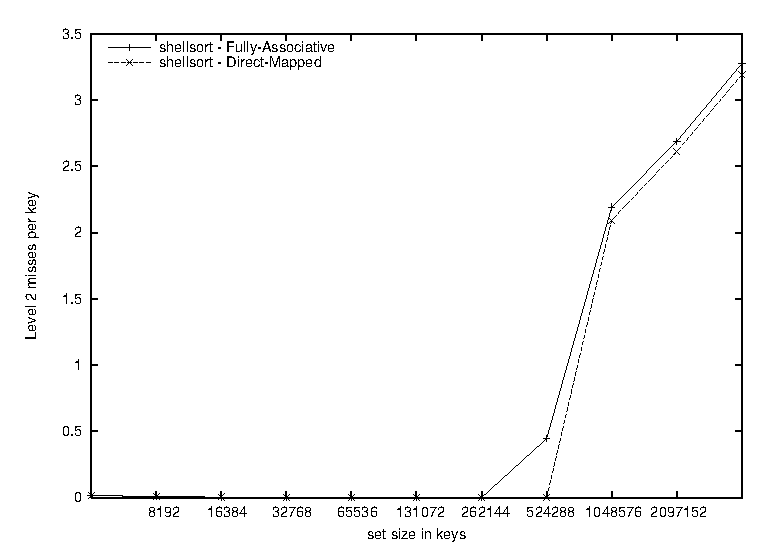
\includegraphics[scale=\subscale]{plots/cache_misses_level_2_shell.eps}}
\subfigure[Caption2]{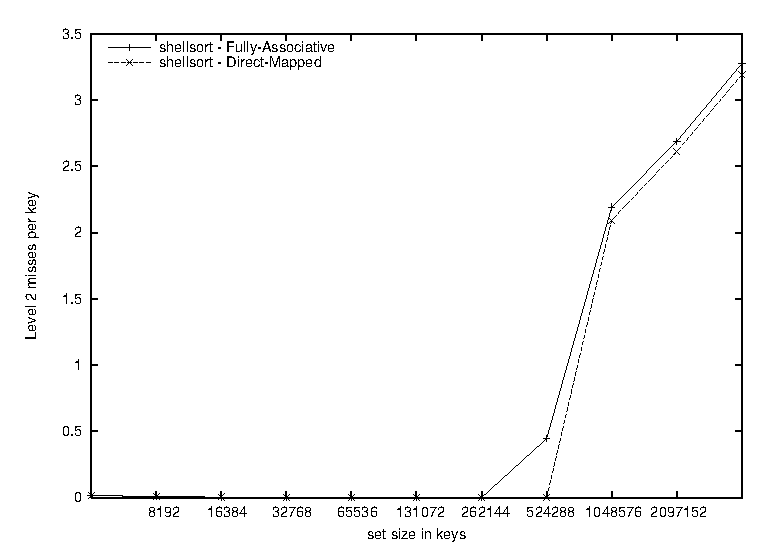
\includegraphics[scale=\subscale]{plots/cache_misses_level_2_shell.eps}}
\caption{TODO: Predictability of insertion and selection sorts}
\label{Cache-misses-in-shellsort}
\end{figure}


\section{Heapsort}
Heapsort is an in-place sort which works in $O(NlogN)$ time in the
average and worst case. It begins by creating a structure known as a
heap, a binary tree in which a parent is always larger its child,
and the largest key is at the top of the heap. It then repeatedly
removes the largest key from the top and places it in its final
position in the array, fixing the heap as it goes.


\section{Quicksort}
Quicksort is a divide and conquer algorithm that recursively
partitions its array around a pivot, swapping large keys on the left
hand side with smaller keys on the right hand side. The partition
causes the pivot to be put in its final position, with all greater
keys to the right, and lesser keys on the left. The left and right
partitions are then sorted recursively.

\subsection{Simple Quicksort}
Sedgewick \cite{} has proposed a number of improvements to the
standard quicksort algorithm, which we use in our base quicksort
implementation. First, we use an explicit stack to save space.
Secondly, we always sort the smaller partition of the array first, to
reduce the worst case size of the stack (from $O(N)$ to
$O(logN)$). Thirdly, we not quicksort patitions of less than a certain
\texttt{THRESHOLD} size; instead we do a final insertion pass over the
array after quicksorting. The smallest of the first \texttt{THRESHOLD}
keys is placed in the first location of the array as a
sentinel. Finally, we use median-of-3 to select the pivot, which
greatly reduces the likelihood of very unbalanced partitioning. This
also allows the bounds check to be removed from the inner loop,
greatly reducing the instruction count. Improvements such as these are
found in most efficient implementations of quicksort.

In addition to our base quicksort algorithm, we experimented with
variations which attempt to reduce the number of data cache
misses. LaMarca \cite{} proposed a \textit{memory-tuned} quicksort.
Once a partition is reduced below the size of the threshold, insertion
sort is preformed immediately. By doing this, the keys being sorted
are in the cache already. By leaving the insertion sort until the end,
as Sedgewick does, the reduction in instruction count is made up by
the increase in cache misses, once the lists being sorted are larger
than the cache.

\subsection{Multi-Quicksort}
Generally, quicksort has good locality of reference. It divides the
same region of the array into increasingly small partitions.  In the
case that the array to be sorted fits in a particular level of the
cache, then quicksort has excellent cache properties at that
level. Once the array is larger than the cache, however, the number of
misses increases dramatically. On the early passes, which divide the
array into large sections, there is likely to be little reuse of data
cache entries between passes. Given that there is little reuse between
passes, it would be better to reduce the number of passes by dividing
the array into a larger number of partitions on each pass. LaMarca
uses a technique similar to that used in multi-mergesort, in that a
multi-way partition is done at the start, moving all keys into
cache sized containers which can be sorted individually.

Implementing a multi-way partition is complicated. At the start of the
algorithm, a set of pivots is chosen and sorted, and keys are put into
containers based on which two pivots their value lies between. A
minimal and maximal key are put on the edges of this list to avoid
bounds checks as the list is iterated over.

The main problem with multi-quicksort is that we don't know how many
keys there will be in each container. We implement the containers as a
linked list of arrays. LaMarca notes very little performance
difference between 100 and 5000 keys in each block. The size is
therefore chosen so that each list fits exactly into a page of
memory. When a list is filled, another list is linked to it, and these
lists hold all the keys in the container. The total number of
containers is chosen so that on average each will hold $C/3$ keys,
where $C$ is the number of keys which fit in the cache. LaMarca shows
that using this formula on average only 5\% of subsets will be larger
than the cache.

The entire array is iterated though a key at a time. For each key, the
list of pivots are searched until the appropriate container is found,
and the key is added to that container. Sequentially searching the
lists increases the instruction count by 50\% over the memory-tuned
version. For this reason, the search was replaced with an efficient
binary search, which reduced by half the extra instructions.

Once the entire array has been put into containers, each container is
emptied in turn and the keys put back into the array. When a container
is empty, the pivot greater than that container is put into position,
which is guaranteed to be its final position. The indices of these
positions is pushed onto the stack, and the sub-array is then sorted.

While emptying the containers back into the array, an opportunity is
taken to find the smallest key in the leftmost partition. This is
placed as a sentinel, ensuring that every partition has a sentinel,
and that no bounds checks are required.

\subsection{Quicksort Results}
Figure \ref{} shows the 




\section{Radixsort}



\section{Related work} 

% The IBM 7030 "Stretch" supercomputer was the first general-purpose
% pipelined architecture \cite{Bloch59}. Released in 1959 it had a
% four-stage pipeline and many other architectural innovations that are
% now commonplace in desktop and even embedded computers. 

We present the first large-scale systematic study of branch prediction
and sorting. However, researchers have been aware for many years that
the branches in comparison-based sorts cause problems on pipelined
architectures. As early as 1972 Knuth commented on the
'ever-increasing number of "pipeline" or "number crunching" computers
that have appeared in recent years' whose 'efficiency deteriorates
noticeably in the presence of conditional branch instructions unless
the branch almost always goes the same way'. He also notes that 'radix
sorting is usually more efficient than any other known method for
internal sorting on such machines' \cite{Knuth72c}. Most likely, Knuth
was referring to the IBM 7030 "Stretch" computer (released in 1961
with a four-stage pipeline), Seymor Cray's Freon-cooled CDC 6600
supercomputer (released 1964), or other early supercomputers which
used pipelining in the execution of general-purpose instructions.

A number of other authors have considered optimized implementations of
sorting algorithms for more recent single-processor machines. Nyberg
et al present a quicksort-based algorithm for RISC architectures
\cite{Nyberg+94}. They found that the main limit on performance was
cache behaviour, and did not mention branch prediction even
once. Bentley implemented a highly-tuned quicksort, to be used in the
\texttt{qsort} function of the standard C library
\cite{Bentley93}. Again, Bentley did not consider branch prediction,
perhaps because the first desktop processors with dynamic branch
predictors (such as the DEC Alpha 21064, MIPS R8000 and Intel Pentium)
were only just appearing around that time.

Agarwal developed an optimized algorithm for sorting random records on
an IBM RS/6000 RISC machine \cite{Agarwal96}. His is the first
published algorithm that we are aware of that deliberately attempts to
improve performance by eliminating branch mispredictions. First, it
uses the seven higher order bits of the key to divide the data into
128 buckets. Each of these buckets is radix-sorted. However, before
the radix sort is reaches the lowest order bits, the probability of
any adjacent pair of keys being out of order is extremely low, because
the problem states that the data is guaranteed to be random. In the
final stage, the algorithm checks that large runs of keys are
correctly ordered using subtraction and bitwise operations, and only
sorts a section if some key is found to be out of order. Although
Agarwal's techniques are interesting, they are very dependent on the
randomness of the data; it is easy to construct commmon cases that
would result in very poor performance. Nonetheless, the work is
interesting because it shows the effectiveness of radix sorting
techniques on pipelined architectures.

A recent trend in optimizing algorithms for FFT, linear algebra, and
digital signal processing has been to automatically generate and
evaluate very large numbers of variants of the algorithm.  A similar
approch is used by \cite{Li+05} to automatically generate sorting
algorithms that are tuned to the architecture of the target machine
and the characteristics of the input data. They identify six sorting
primitives, which can be combined to construct a sorting algorithm.  A
large number of combinations are tested, using a genetic algorithms
search to find the most efficient. The resulting implementations are,
in many cases, significantly faster than commercial sorting libraries.
Although they do not consider branch prediction explicitly, they find
that the implementations that perform best usually use radix sort for
a large part of the sorting process.

Sanders and Winkel investigate the use of \emph{predicated}
instructions on Intel Itanium~2 processors \cite{SandersWinkel05}. In
addition to its normal inputs, a predicated instruction takes a
predicate register input. If the value in the predicate register is
true, the instruction takes effect; otherwise it does not. Predication
is normally implemented by the instruction being executed regardless
of whether the predicate is true. However, its result is only
\textit{written back} to a register or memory if the predicate is
true. Although predicated instructions use execution resources
regardless of whether they are allowed to write back, they allow
conditional branches to be eliminated.  Sanders and Winkel show how
the partition step in quicksort can be rewritten to use predicated
instructions on an Itanium~2 highly instruction-level parallel
machine. Itannium~2 provides large numbers of parallel functional
units and registers which make such trade-offs worthwhile.

We attempted to replicate Sanders and Winkel's work a Pentium~4 based
desktop machine, using conditional move instructions (the only form of
predicated instructions on the Pentium~4). The standard form of the
quicksort loops is highly efficient, but we found that rewriting them
into a single loop suitable for predication made them less so. The
transformation also increased the number of simultaneously live
values, which exceeded the number of available registers. We also
discovered that, at least on the Pentium 4, conditional moves are
surprisingly expensive.

Mudge \textit{et al} examine the behaviour of the $i$ and $j$
comparison branches in quicksort, as an example to demonstrate a
general method for estimating the limit on the predictability of
branches in a program \cite{Mudge+96}. They argue that the optimal
predictor for these branches would keep a running count of the total
number of the proportion of array elements examined so far that are
greater than the pivot. They estimate that this approach will give a
prediction accuracy of around 75\%, which is remarkably close to our
result for these branches, using a bimodal predictor.

\textbf{Describe the paper from Alenex 2005}

To our knowlege, this is the only research, other than our own, that
investigates and attempts to understand the predictability of
comparison branches in sorting, rather than simply attempting to
eliminate such branches.


\section{Conclusions}


\comment{
\begin{acks}
We would like to thank the anonymous reviewers of VEE 2005, whose
comments greatly improved an earlier version of this paper.
\end{acks}
}

\bibliographystyle{acmtrans}
\bibliography{report}
%\begin{thebibliography}{...}
%\end{thebibliography}

\begin{received}
...
\end{received}
\end{document}


